\documentclass[a4paper, twoside]{report}

%% Language and font encodings
\usepackage[english]{babel}
\usepackage[utf8x]{inputenc}
\usepackage[T1]{fontenc}

%% Sets page size and margins
\usepackage[a4paper,top=3cm,bottom=2cm,left=3cm,right=3cm,marginparwidth=1.75cm]{geometry}

%% Useful packages
\usepackage{amsmath, amsfonts}
\usepackage{graphicx}
\usepackage[colorinlistoftodos]{todonotes}
\usepackage[colorlinks=true, allcolors=blue]{hyperref}

\usepackage{tikz}
\usepackage{booktabs}
\usepackage{listings}
\usetikzlibrary{arrows.meta}
\tikzset{%
  % Specifications for style of nodes:
            base/.style = {rectangle, rounded corners, draw=black,
                           minimum width=4cm, minimum height=1cm,
                           text centered, font=\sffamily},
  activityStarts/.style = {base, fill=blue!30},
       startstop/.style = {base, fill=red!30},
    aggclustering/.style = {base, fill=green!30},
         process/.style = {base, minimum width=2.5cm, fill=orange!15,
                           font=\ttfamily},
}

\newcommand\mydot[1][.5]{{\vcenter{\hbox{\scalebox{#1}{$\bullet$}}}}}


\title{Statistical cyber-security: Searching for patterns in commands issued by malicious intruders}
\author{Hanyang Liu}
% Update supervisor and other title stuff in title/title.tex

\begin{document}
\begin{titlepage}

\newcommand{\HRule}{\rule{\linewidth}{0.5mm}} % Defines a new command for the horizontal lines, change thickness here

%----------------------------------------------------------------------------------------
%	LOGO SECTION
%----------------------------------------------------------------------------------------


\includegraphics[width=8cm]{title/logo.eps}\\[1cm] % Include a department/university logo - this will require the graphicx package
 
%----------------------------------------------------------------------------------------

\center % Center everything on the page

%----------------------------------------------------------------------------------------
%	HEADING SECTIONS
%----------------------------------------------------------------------------------------

\textsc{\LARGE Undergraduate Research Opportunities Programme}\\[1.5cm] % Name of your university/college
\textsc{\Large Imperial College London}\\[0.5cm] % Major heading such as course name
\textsc{\large Department of Mathematics}\\[0.5cm] % Minor heading such as course title

%----------------------------------------------------------------------------------------
%	TITLE SECTION
%----------------------------------------------------------------------------------------
\makeatletter
\HRule \\[0.4cm]
{ \huge \bfseries \@title}\\[0.4cm] % Title of your document
\HRule \\[1.5cm]
 
%----------------------------------------------------------------------------------------
%	AUTHOR SECTION
%----------------------------------------------------------------------------------------

\begin{minipage}{0.4\textwidth}
\begin{flushleft} \large
\emph{Author:}\\
\@author % Your name
\end{flushleft}
\end{minipage}
~
\begin{minipage}{0.4\textwidth}
\begin{flushright} \large
\emph{Supervisor:} \\
Prof. Nick Heard \\ % Supervisor's Name
Dr. Francesco Sanna Passino % second supervisor's name
\end{flushright}
\end{minipage}\\[2cm]
\makeatother

% If you don't want a supervisor, uncomment the two lines below and remove the section above
%\Large \emph{Author:}\\
%John \textsc{Smith}\\[3cm] % Your name

%----------------------------------------------------------------------------------------
%	DATE SECTION
%----------------------------------------------------------------------------------------

{\large \today}\\[2cm] % Date, change the \today to a set date if you want to be precise

\vfill % Fill the rest of the page with whitespace

\end{titlepage}

\begin{abstract}
    Artificial intelligence is an active research and development area within cyber-security. 
    The potential to automatically detect intruders within a computer network by building sophisticated, 
    time-varying statistical models of their evolving behaviours, 
    allowing outlying anomalous behaviours to be identified, 
    has attracted much interest from industry and government. 
    Less attention has been paid to modelling the actions and objectives of network intruders,
    largely due to a lack of available data containing known malicious behaviour.
    In this paper, we propose a method to use hierarchical agglomerative clustering
    and multinomial-dirichlet distribution to cluster the sessions of commands.
    The clustering successfully reduces dimensions while
    maintaining expected predictive probability.
\end{abstract}

% \renewcommand{\abstractname}{Acknowledgements}
% \begin{abstract}
% Thanks mum!
% \end{abstract}

\tableofcontents
\listoffigures
\listoftables

\chapter{Introduction}
\section{Objectives}
Artificial intelligence is an active research and development area within cyber-security. 
The potential to automatically detect intruders within a computer network by building sophisticated, 
time-varying statistical models of their evolving behaviours, 
allowing outlying anomalous behaviours to be identified, 
has attracted much interest from industry and government. 
Less attention has been paid to modelling the actions and objectives of network intruders,
largely due to a lack of available data containing known malicious behaviour.
This project will investigate a new data resource, 
where in collaboration with Microsoft a so-called “honeypot” has been planted in the college network 
to entice network intruders and record their actions. 
Discoveries from this research theme have the potential 
to provide enterprise situational awareness of the intentions of an intruder detected on a network, 
allowing a targeted response such as preventing access to the most sensitive data held by an organisation.

\section{Related Work}
Some work \cite{sadique2021analysis}studies ways to predict attackers' next commands from the shell commands
using Levenshtein distance without analyzing network traffic.
\chapter{Background}

\section{Exploratory Data Analysis}
There are 124883 out of 125280 sessions which appear only once in the Microsoft dataset.
The dataset can be found in Appendix \ref{tab:headdf} and sessions look like Appendix \ref{lst:sessions}.
If we divide sessions into sequences of commands of length 12\cite{sadique2021analysis},
many sequences seem to be naturally clustered by frequncies of appearance, as shown in Fig \ref{fig:EDA}.
Within each cluster, not only the distribution of initial few commands seem very homogeneous,
but also the sequences themselves.
\begin{figure}[h]
    \centering
    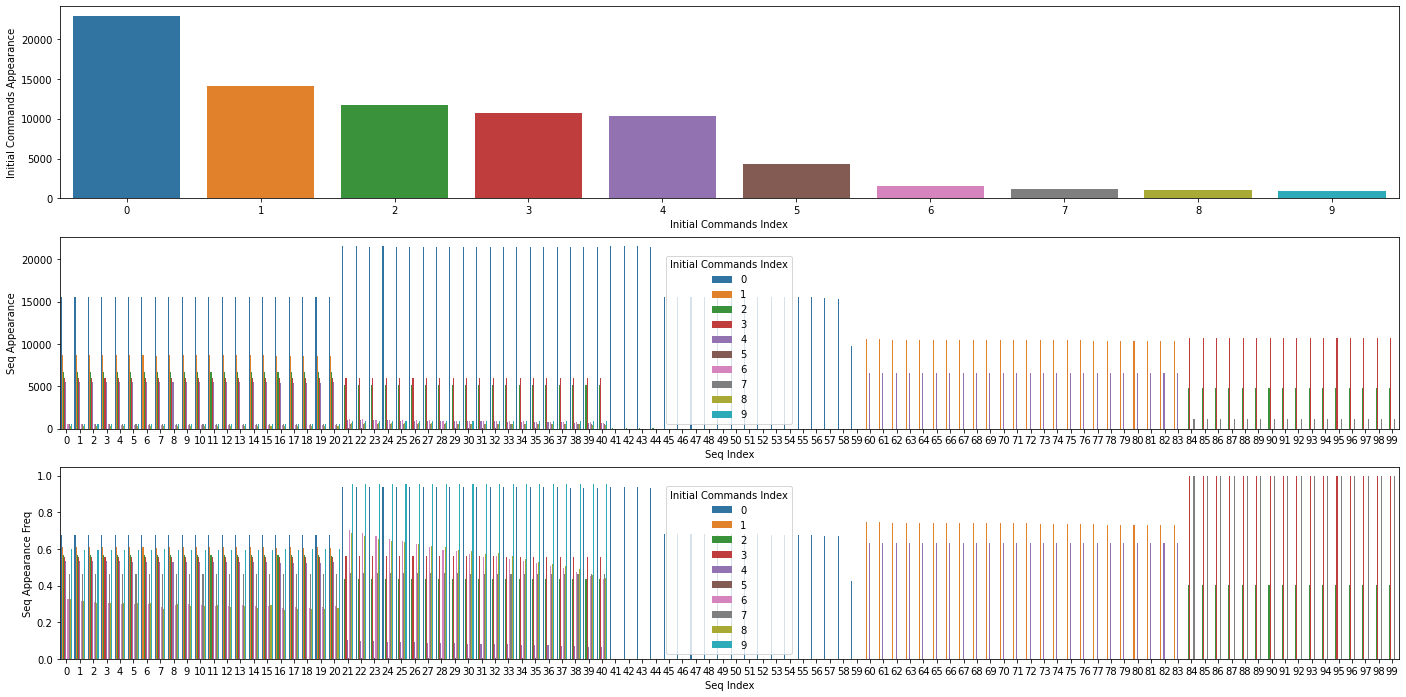
\includegraphics[scale=0.3]{background/EDA.png}
    \caption{Exploratory Data Analysis. The top graph shows the number of appearance of 
    top 10 frequent initial 3 commands. The middle graph shows the number of appearance of 
    top 10 frequent initial 3 commands in sessions which contain top 100 frequent sequence of commands.
    The bottom graph shows the frequency of top 10 frequent 
    initial 3 commands in sessions which contain top 100 frequent sequence of commands}
    \label{fig:EDA}
\end{figure}
\\
This encourages us to try to cluster and predict the commands based on the initial commands in a session.
\section{Data Pre-processing}
There are 3 major objectives in data processing.
\begin{enumerate}
    \item Seperate multiple commands in one command line.
    \item Use \textbf{r'[a-zA-Z0-9\_$\backslash$.$\backslash$-$\backslash$*]+'} as regexp to tokenise commands into words.
    \item Replace the words which only appear in one session by rarecommand.
\end{enumerate}
The sample code can be found in Appendix \ref{lst:tokeniser}
\section{Hierarchical Agglomerative Clustering}
Hierarchical clustering is a method which exhaustively merge pairs of clusters.
Each observation starts in its own cluster. 
Iteratively, the closest (most similar) pairs of clusters merge, 
until there is only one cluster or the threshold is achived.
\chapter{Model}

\section{Clustering}
We aim to cluster sessions and predict commands based on the first \(d\) commands of each session.
Therefore, the model can be divided into clustering part and prediction part.
\\\\
We need to assign each session a label, so that we can evaluate how homogeneous each cluster is,
and we can use the labels as surrogates for predictions.
We divide sessions into sequences of commands of length \(l_c\)\cite{sadique2021analysis}.
For example, if a session is \textbf{A-B-C-D-E-F} and \(l_c=3\), 
we will have sequences \textbf{A-B-C}, \textbf{B-C-D}, \textbf{C-D-E}, and \textbf{D-E-F}.
Sequences of commands are ranked by their number of appearances, 
i.e. the most frequent sequence is ranked 1, the second most frequent sequence is ranked 2.
For each session \(x\), we assign label \(y\) as the highest rank which can be achieved by the sequences obtained from \(x\).
We denote \(x_{j}\) to be the \(j\)th command of \(x\),
and \(x_{:d}\) to be the initial \(d\) commands of \(x\).
Suppose we have \(N\) unique initial \(d\) commands and the lowest rank of our sessions is \(K\),
an \(N\) by \(K\) matrix of counts \(A\) can be constructed as following: 
\(A_{pq}\) is the number of sessions \(x\) for which \(x_{:d}\) is the \(p\)th unique first \(d\) commands,
and \(y=q\).
\\\\
Hierarchical Agglomerative Clustering method is used for our clustering.
The idea is that we start with \(N\) clusters, and pairwisely
merge closest clusters in a predefined metric until certain threshold.
In our case, for each initial cluster \(p\), we assume that the unknown categorical probability
$\theta=(\theta_1,\ldots,\theta_K)$ follows a Dirichlet prior,
\begin{equation}
    \theta\sim \textnormal{Dirichlet}(\beta_1,\ldots,\beta_K),
\end{equation}
with each $\beta_j>0$. Hence we can calculate \(P(A_{p,:}|\theta)\).
Let us define \(E\) as the dissimilarity matrix among clusters.
We then use \(E_{pq}=\log(P(A_{p,:}, A_{q,:}|\theta)) - \log(P(A_{p,:}|\theta)) - \log(P(A_{q,:}|\theta))\)
to calculate the gain in similarity after merging the cluster \(p\) and \(q\). 
Finally, we can perform the agglomerative clustering as usual. 
We use minimum linkage for agglomerative clustering.

\section{Prediction}
We now come to prediction after finishing clustering.
Suppose a particular cluster contains $M\leq N$ data points, corresponding to data matrix row positions $i_1,\ldots,i_M$ of the $N\times K$ data matrix of counts $A=(a_{ij})$. For $1\leq j \leq K$, let
\begin{equation}
  n_j = \sum_{\ell=1}^M a_{i_\ell j}
\end{equation}
be the total frequency of category $j$ in the cluster, and let $n_{\mydot} =\sum_j n_j$. Suppose the unknown categorical probabilities $\theta=(\theta_1,\ldots,\theta_K)$ for the cluster follow a Dirichlet prior,
\begin{equation}
  \theta\sim \textnormal{Dirichlet}(\alpha_1,\ldots,\alpha_K),
\end{equation}
with each $\alpha_j>0$ and $\alpha_{\mydot} = \sum_j \alpha_j$.
Then the marginal likelihood of the sequence of observed categories which gave rise to the bin frequencies $n_1,\ldots,n_k$ is
\begin{equation}
  \frac{\Gamma(\alpha_{\mydot})}{\Gamma(\alpha^\ast_{\mydot})}\prod_{j=1}^K \frac{\Gamma(\alpha^\ast_j)}{\Gamma(\alpha_j)},
\end{equation}
where $\alpha^\ast_j=\alpha_j + n_j$ for $1\leq j \leq K$ and $\alpha^\ast_{\mydot}=\sum_j \alpha^\ast_j=\alpha_{\mydot}+n_{\mydot}$.
Furthermore, the posterior distribution for $\theta$ after observing $n_1,\ldots,n_K$ is
\begin{equation}
  \theta\mid n_1,\ldots,n_K \sim \textnormal{Dirichlet}(\alpha^\ast_1,\ldots,\alpha^\ast_K).
\end{equation}
In particular, this means
\begin{equation}
  \mathbb{E} (\theta_j \mid n_1,\ldots,n_K) = \frac{\alpha^\ast_j}{\alpha^\ast_{\mydot}}.\label{eq:predictive}
\end{equation}
The quantity \eqref{eq:predictive} is also the predictive probability for category $j$ in that cluster. So if we have a new observation assigned to the cluster with label $y_{N+1}$, the prediction score we get from that observation is
\begin{equation}
  \frac{\alpha^\ast_{y_{N+1}}}{\alpha^\ast_{\mydot}}.
\end{equation}
For each leaf node, the expected predictive probability in that cluster is
\begin{equation}
    \mathbb{E} (p(x)) = \sum_{j=1}^K (\frac{\alpha^\ast_j}{\alpha^\ast_{\mydot}})^2.
\end{equation}
Therefore, we can calculate the weighted sum of the expected predictive probabilities across the clusters,
where the cluster weight is proportional to the number of observations in that cluster.
This can be an indication of our overall cluster result.

\section{Model Architecture}
We can now combine the clustering and prediction part to construct our model.
Suppose we want to train depth \(d\), 
which means we know the initial \(d\) commands of all sessions to help us cluster.
\begin{figure}[h]
    \centering
    \scalebox{.8}{\tikzset{%
  % Specifications for style of nodes:
            base/.style = {rectangle, rounded corners, draw=black,
                           minimum width=4cm, minimum height=1cm,
                           text centered, font=\sffamily},
  activityStarts/.style = {base, fill=blue!30},
       startstop/.style = {base, fill=red!30},
    aggclustering/.style = {base, fill=green!30},
         process/.style = {base, minimum width=2.5cm, fill=orange!15,
                           font=\ttfamily},
}
% Drawing part, node distance is 1.5 cm and every node
% is prefilled with white background

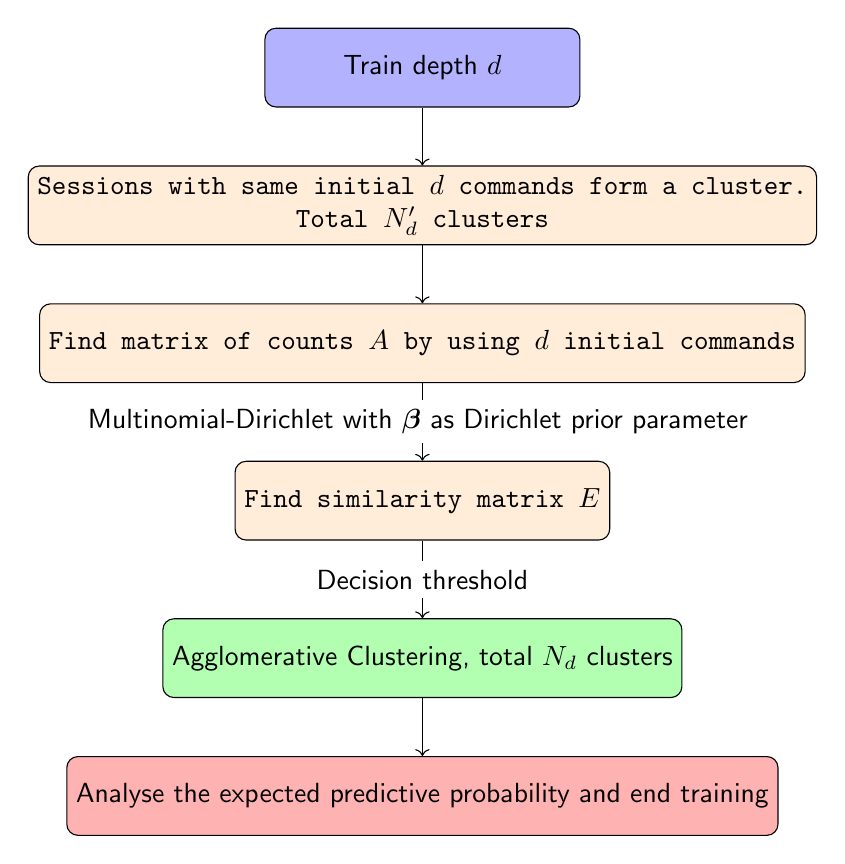
\begin{tikzpicture}[node distance=1.5cm,
    every node/.style={fill=white, font=\sffamily}, align=center]
  % Specification of nodes (position, etc.)
  \node (start)             [activityStarts]              {Train depth \(d\)};

  \node (ncluster)      [process, below of=start, yshift=-0.25cm] 
  {Sessions with same initial \(d\) commands form a cluster.\\Total \(N_d'\) clusters};
  \node (matA)     [process, below of=ncluster, yshift=-0.25cm]          
  {Find matrix of counts $A$ by using \(d\) initial commands};
  \node (matE)      [process, below of=matA, yshift=-0.5cm]   
  {Find similarity matrix $E$};
  \node (aggclustering2)      [aggclustering, yshift=-0.5cm,below of=matE]  
  {Agglomerative Clustering, total \(N_d\) clusters};
  \node (end)      [startstop, yshift=-0.25cm,below of=aggclustering2]  
  {Analyse the expected predictive probability and end training};
  % Specification of lines between nodes specified above
  % with aditional nodes for description 
  \draw[->]      (start) -- (ncluster);
  \draw[->]      (ncluster) -- (matA);
  \draw[->]     (matA) -- node[]{
      Multinomial-Dirichlet with \(\boldsymbol{\beta}\) as Dirichlet prior parameter
  }(matE);
  \draw[->]      (matE) -- node[]{Decision threshold}(aggclustering2);

  \draw[->]      (aggclustering2) -- (end);
\end{tikzpicture}}
    \caption{Flowchart of Intuitive Model}
    \label{fig:model1}
\end{figure} 
The intuitive way of combination is like Fig \ref{fig:model1}. 
However, the main drawback is that it cannot learn from previous clustering.
For example, the initial 7 commands \textbf{A-B-C-D-E-F-G} and \textbf{A-B-C-D-E-F-H}
are completely different in the intuitive model. 
The initial 6 commands, however, are considered same.
Many times the command \textbf{G} and \textbf{H} may only differ by a URL.
Treating \textbf{A-B-C-D-E-F-G} and \textbf{A-B-C-D-E-F-H} and \textbf{I-I-I-I-I-I-I} 
as 3 completely different cluster is not reasonable.
\\\\
Therefore, we propose a model which can both combine clustering and prediction, and learn from previous depth.
\begin{figure}[h]
    \centering
    \scalebox{.8}{\tikzset{%
  % Specifications for style of nodes:
            base/.style = {rectangle, rounded corners, draw=black,
                           minimum width=4cm, minimum height=1cm,
                           text centered, font=\sffamily},
  activityStarts/.style = {base, fill=blue!30},
       startstop/.style = {base, fill=red!30},
    aggclustering/.style = {base, fill=green!30},
         process/.style = {base, minimum width=2.5cm, fill=orange!15,
                           font=\ttfamily},
}
% Drawing part, node distance is 1.5 cm and every node
% is prefilled with white background

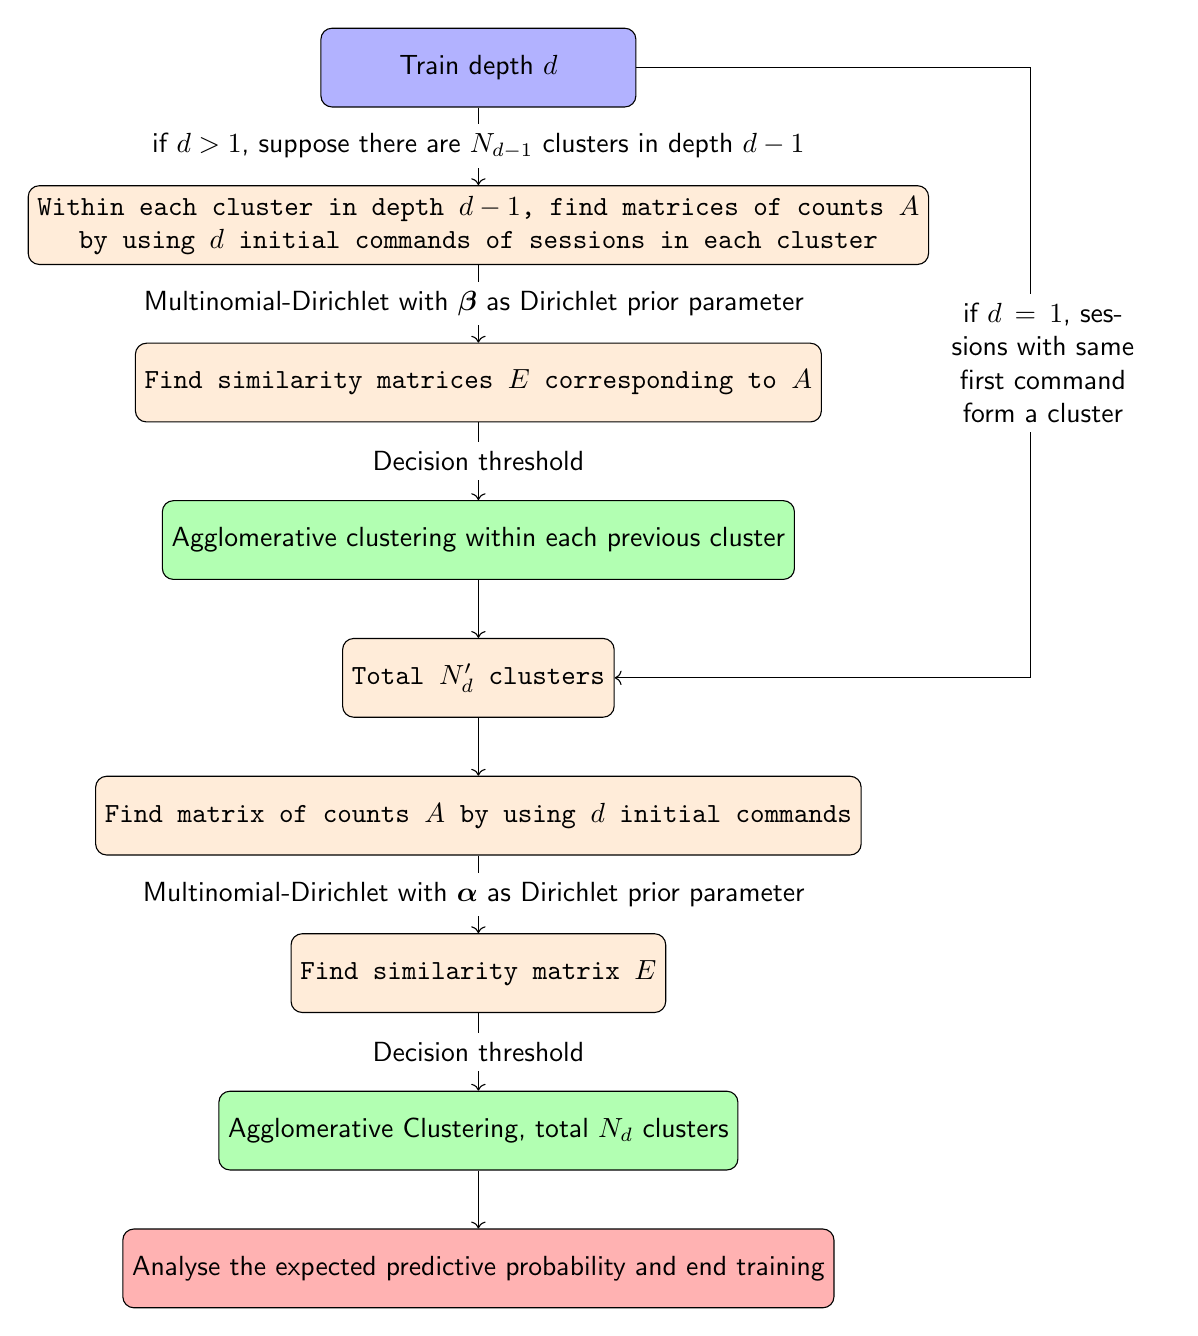
\begin{tikzpicture}[node distance=1.5cm,
    every node/.style={fill=white, font=\sffamily}, align=center]
  % Specification of nodes (position, etc.)
  \node (start)             [activityStarts]              {Train depth \(d\)};
  \node (matAs)     [process, below of=start, yshift=-0.5cm]          
  {Within each cluster in depth \(d-1\), find matrices of counts $A$\\
  by using \(d\) initial commands of sessions in each cluster};
  \node (matEs)      [process, below of=matAs, yshift=-0.5cm]   
  {Find similarity matrices $E$ corresponding to \(A\)};
  \node (aggclustering)      [aggclustering, yshift=-0.5cm,below of=matEs]  
  {Agglomerative clustering within each previous cluster};
  \node (ncluster)      [process, below of=aggclustering, yshift=-0.25cm] 
  {Total \(N_d'\) clusters};
  \node (matA)     [process, below of=ncluster, yshift=-0.25cm]          
  {Find matrix of counts $A$ by using \(d\) initial commands};
  \node (matE)      [process, below of=matA, yshift=-0.5cm]   
  {Find similarity matrix $E$};
  \node (aggclustering2)      [aggclustering, yshift=-0.5cm,below of=matE]  
  {Agglomerative Clustering, total \(N_d\) clusters};
  \node (end)      [startstop, yshift=-0.25cm,below of=aggclustering2]  
  {Analyse the expected predictive probability and end training};
  % Specification of lines between nodes specified above
  % with aditional nodes for description 
  \draw[->]             (start) -- node[] 
                                    {if \(d>1\), suppose there are \(N_{d-1}\) clusters in depth \(d-1\)}(matAs);
  \draw[->]     (matAs) -- node[]{
      Multinomial-Dirichlet with \(\boldsymbol{\beta}\) as Dirichlet prior parameter
  }(matEs);
  \draw[->]      (matEs) -- node[]{Decision threshold}(aggclustering);
  \draw[->]      (aggclustering) -- (ncluster);
  \draw[->] (start.east) -- ++(5,0) -- ++(0,-7.75)  --                
  node[xshift=2.8cm, yshift=4cm, text width=3cm]
  {if \(d=1\), sessions with same first command form a cluster}(ncluster.east);
  \draw[->]      (ncluster) -- (matA);

  \draw[->]     (matA) -- node[]{
      Multinomial-Dirichlet with \(\boldsymbol{\alpha}\) as Dirichlet prior parameter
  }(matE);
  \draw[->]      (matE) -- node[]{Decision threshold}(aggclustering2);

  \draw[->]      (aggclustering2) -- (end);
\end{tikzpicture}
}
    \caption{Flowchart of Our Model}
    \label{fig:model2}
\end{figure}
Suppose we want to cluster in depth \(d\).
As shown in Fig \ref{fig:model2}, the idea we introduce is to cluster within each previous cluster in depth \(d-1\) first.
After this is done, we try to see if the existing clusters can be further combined.
This assymetric clustering procedure gives advantage to sessions with different initial \(d\) commands,
but in the same cluster in depth \(d-1\).    

\chapter{Evaluation}
We set our Dirichlet prior \(\boldsymbol{\alpha}\) and \(\boldsymbol{\beta}\) to be 
0.0001 in all categories, given we have investigated that \(K\),
the size of categories in a cluster, is around 1000 for this dataset.
The cluster threshold we use is \(0.3\).
We also experiment different length of sequence of commands, \(l_c\).
\\\\
In order to evaluate our performance, we design 2 baselines using \(l_c=12\) to calculate matrices \(A\) and \(E\). 
\textbf{Baseline 1} is to keep every unique initial \(d\) commands in its own clusters for depth \(d\).
\textbf{Baseline 2} is to put all observations into a single cluster, i.e. not doing any clustering.
\begin{table}[h]
    \centering
    \begin{tabular}{lllllll}
\toprule
{} &   Depth 1 &   Depth 2 &   Depth 3 &   Depth 4 &   Depth 5 &   Depth 6 \\
\midrule
$l\_c=3$    &  0.476399 &  0.524108 &  0.539341 &  0.547319 &  0.551775 &  0.555026 \\
$l\_c=6$    &  0.460124 &   0.50814 &  0.524318 &  0.532581 &  0.536925 &  0.546313 \\
$l\_c=9$    &  0.453345 &  0.501228 &  0.527811 &  0.536087 &  0.541361 &   0.55031 \\
$l\_c=12$   &  0.450155 &   0.49781 &  0.530307 &  0.538657 &  0.544359 &   0.55324 \\
Baseline 1 &  0.454241 &  0.517255 &  0.549589 &  0.568437 &  0.574061 &  0.603752 \\
Baseline 2 &  0.432368 &        NA &        NA &        NA &        NA &        NA \\
\bottomrule
\end{tabular}

    \caption{Expected predictive probabilities}
    \label{tab:prob_df}
\end{table}
\begin{table}[h]
    \centering
    \begin{tabular}{lllllll}
\toprule
{} & Depth 1 & Depth 2 & Depth 3 & Depth 4 & Depth 5 & Depth 6 \\
\midrule
$l\_c=3$    &      11 &      41 &      66 &      76 &      80 &      89 \\
$l\_c=6$    &      14 &      48 &      71 &      81 &      94 &     104 \\
$l\_c=9$    &      14 &      48 &      73 &      82 &      95 &     101 \\
$l\_c=12$   &      14 &      47 &      69 &      81 &      95 &     102 \\
Baseline 1 &    1796 &    7380 &   14237 &   19537 &   19931 &   28116 \\
Baseline 2 &       1 &      NA &      NA &      NA &      NA &      NA \\
\bottomrule
\end{tabular}

    \caption{Number of clusters}
    \label{tab:cluster_df}
\end{table}
\\
Table \ref{tab:prob_df} shows the result of our expected predictive probabilities.
Table \ref{tab:cluster_df} shows the result of number of clusters.
For Baseline 1, as the number of clusters grows drastically fast as depth increases,
most clusters will have very few elements, except for the few dominant ones.
Therefore, we have many small homogeneous clusters in Baseline 1
and we can expect the expected predictive probabilities increases as depth increases.
For Baseline 2, it is meaningless to talk about depth as we put all observations into a single cluster.
its expected predictive probability is lowest among all, as we expect.
However, even if we put all obervations into 1 single cluster,
the expected predictive probability, 0.432368, is still quite high.
This can be due to the imbalance of dataset which can limit our performance gain as depth increases.
\\\\
A sample clustering of initial commands can be found in Appendix \ref{lst:cluster}.
We can see that for each \(l_c\), the expected probabilities increase as depth increases,
and the numbers of clustering are much fewer than Baseline 1.
\chapter{Conclusion}
The result shows that our method can successfully allocate the sessions of commands
from thousands of initial clusters to fewer than 100 clusters,
while maintaining the expected predictive probability.

\appendix
\chapter{Appendix}
Details of code can be found in \href{https://github.com/Hanyang97/UROP}{https://github.com/Hanyang97/UROP}
\\
\begin{table}[h]
    \centering
    \begin{tabular}{llllrllr}
\toprule
{} & Protocol &                                           Commands &                                                 ID &  TimesSeen &                FirstSeen &                 LastSeen \\
\midrule
0 &   Telnet &  [enable, system... &  14cc70cddce... &    1546097 &  2019-07-...&   2019-11-...\\
1 &   Telnet &  [enable, system ... &  ba4417b91e... &    1149119 &  2019-07-...&  2019-09-...\\
2 &   Telnet &  [sh, ... &  e421974df... &    1279661 &   2019-07-...&  2019-09-...\\
3 &   Telnet &  [sh, bin... &  5d9c6f7... &     346137 &  2019-07-...&  2019-11-...\\
4 &   Telnet &  [shell, sh... &  0d1edf8dad... &    2435245 &  2019-07-...&  2019-11-...\\
\bottomrule
\end{tabular}

    \caption{Microsoft honeypot dataset}
    \label{tab:headdf}
\end{table}

\begin{lstlisting}[language=Python, caption={Python code for tokeniser}, label={lst:tokeniser},captionpos=b]
    from nltk.tokenize import RegexpTokenizer
    from gensim.corpora import Dictionary
    
    
    def clean_commands(dat, no_below=2, no_above=1.1):
        """
        This function 
        1. splits multiple commands in the same line
        2. tokenize the commands
        3. replace rare commands by rarecommand
    
        :param dat: dataset
        :param no_below: Keep tokens which are 
            contained in at least no_below documents.
        :param no_above: Keep tokens which are 
            contained in no more than no_above documents 
        (fraction of total corpus size, not an absolute number).
    
        :return sessins_token_list: tokenized list of sessions 
            of commands
        :return dictionary: dictionary generated
        """
        # for commands splitted by ;
        sessions = []
        for session in dat['Commands']:
            sessions.append([])
            for command in session:
                sessions[-1] += command.split('; ')
        # tokenizer
        tokenizer = RegexpTokenizer(r'[a-zA-Z0-9_\.\-\*]+')
        sessions_list = []
        commands_list = []
        for session in sessions:
            sessions_list.append([])
            commands_list.append([])
            for command in session:
                command_token = tokenizer.tokenize(command)
                sessions_list[-1] += [command_token]
                commands_list[-1] += command_token
        dictionary = Dictionary(commands_list)
        dictionary.filter_extremes(no_below, no_above)
        # repleace rare commands by rarecommand
        dictionary.id2token[-1] = 'rarecommand'
        dictionary.token2id['rarecommand'] = -1
        sessions_token_list = []
        for session in sessions_list:
            sessions_token_list.append([])
            commands_token_list = []
            for command in session:
                idxs = dictionary.doc2idx(command)
                commands_token_list.append(
                    ' '.join([dictionary[idx] for idx in idxs]))
            sessions_token_list[-1] += commands_token_list
    
        return sessions_token_list, dictionary
\end{lstlisting}

\begin{lstlisting}[caption={Sample sessions}, label={lst:sessions},captionpos=b]
    ['enable',
    'system',
    'shell',
    'sh',
    '>/tmp/.ptmx && cd /tmp/',
    '>/var/.ptmx && cd /var/',
    '>/dev/.ptmx && cd /dev/',
    '>/mnt/.ptmx && cd /mnt/',
    '>/var/run/.ptmx && cd /var/run/',
    '>/var/tmp/.ptmx && cd /var/tmp/',
    '>/.ptmx && cd /',
    '>/dev/netslink/.ptmx && cd /dev/netslink/',
    '>/dev/shm/.ptmx && cd /dev/shm/',
    '>/bin/.ptmx && cd /bin/',
    '>/etc/.ptmx && cd /etc/',
    '>/boot/.ptmx && cd /boot/',
    '>/usr/.ptmx && cd /usr/',
    '/bin/busybox rm -rf lzrd oxdedfgt',
    '/bin/busybox cp /bin/busybox lzrd; >lzrd; 
    /bin/busybox chmod 777 lzrd; 
    /bin/busybox lizrd',
    '/bin/busybox cat /bin/busybox || while read i; 
    do echo $i; done < /bin/busybox',
    '/bin/busybox lizrd']
\end{lstlisting}

\begin{lstlisting}[caption={Sample cluster sclices}, label={lst:cluster},captionpos=b]
    ('sh',
     'linuxshell',
     'bah',
     'hostname Ex0_1115',
     'bin busybox Ex0',
     'bin busybox ps'),
    ('sh',
     'linuxshell',
     'bah',
     'hostname Ex0_8572',
     'bin busybox Ex0',
     'bin busybox ps'),
    ('sh',
     'linuxshell',
     'bah',
     'hostname Ex0_0447',
     'bin busybox Ex0',
     'bin busybox ps')
\end{lstlisting}


\bibliographystyle{alpha}
\bibliography{bibs/sample}

\end{document}